\documentclass[%
bachelor,    % тип документа
%natbib,      % использовать пакет natbib для "сжатия" цитирований
subf,        % использовать пакет subcaption для вложенной нумерации рисунков
href,        % использовать пакет hyperref для создания гиперссылок
colorlinks,  % цветные гиперссылки
%fixint,     % включить прямые знаки интегралов
]{disser}

\usepackage[
  a4paper,
  mag=1000,
  left=30mm, right=15mm, top=20mm, bottom=20mm,
  headsep=1.25cm,
  footskip=1cm
]{geometry}

\usepackage[intlimits]{amsmath}
\usepackage{amssymb,amsfonts}
\usepackage{icomma}
% Подпись под картинками
\renewcommand\thesubfigure{\asbuk{subfigure}}

\usepackage{float}

\usepackage[T2A]{fontenc}
\usepackage[utf8]{inputenc}
\usepackage[english,russian]{babel}
%!TEX root = thesis.tex"`
\usepackage[acronym,toc]{glossaries}
\makenoidxglossaries

\newacronym{mcc}{MCC}{Multiclass classification}
\newacronym{sshfs}{SSHFS}{SSH File System}
\newacronym{ovr}{OvR}{One-vs.-rest}
\newacronym{vcs}{VCS}{Version Control System}
\newacronym{dag}{DAG}{Directed Acyclic Graph}
\newacronym{nlp}{NLP}{Natural Language Processing}
\newacronym{gb}{Gb}{Gigabyte, 1024 Megabytes}
\newacronym{ovo}{OvO}{One-vs.-one}
\newacronym{tf}{TF}{Term Frequency, частота слова}
\newacronym{idf}{IDF}{Inverse Document Frequency, обратная частота документа}
\newacronym{ml}{ML}{Машинное обучение}
\newacronym{dbms}{DBMS}{Database Management System, также СУБД -- система управления базами данных}
\newacronym{tf-idf}{TF-IDF}{Term frequency - Inverse Document Frequency}
\newglossaryentry{sup_learning}
{
    name=supervised learning,
    description={Постановка задачи, при которой существует т.н. \textit{обучающая выборка}, в которой у каждого элемента известна целевая переменная}
}

\newglossaryentry{semisup_learning}
{
    name=semi-supervised learning,
    description={Постановка задачи, при которой существует выборка, состоящая из $l$ элементов с известной разметкой и $u$ элементов с неизвестной разметкой}
}
\newglossaryentry{unsup_learning}
{
    name=unsupervised learning,
    description={Постановка задачи, при которой не существует выборки с заранее известной целевой переменной}
}
\newglossaryentry{binary_classification}
{
    name=binary classification,
    description={Задача классификации с $\mathbb{Y} = \{0, 1\}$}
}
\newglossaryentry{linear_classifier}
{
    name=linear classifier,
    description={Классификатор вида $y = f\left( \sum\limits_{j}^{} w_j x_j \right)$}
}
\newglossaryentry{svm}
{
    name=support vector machine,
    description={Метод классификации, основанный на пострении разделяющей гиперплоскости так, чтобы отступ от плоскости до объектов разных классов был максимален}
}
\newglossaryentry{soft_margin}
{
    name=soft margin,
    description={Метод классификации, основанный на пострении разделяющей гиперплоскости так, чтобы отступ от плоскости до объектов разных классов был максимален}
}
\newglossaryentry{kernel}
{
    name=kernel,
    description={Функция вида $K(x, y) = \vec{\phi(\vec{x})} \cdot \vec{\phi(\vec{y})}$, использующаяся для улучшения качества на нелинейных зависимостях между входными данными и целевой переменной}
}
\newglossaryentry{hyperparameters}
{
    name=hyperparameters,
    description={Набор численных параметров, которые нельзя оптимизировать на основе обучающей выборки}
}
\newglossaryentry{decision-tree}
{
    name=decision tree,
    description={Алгоритм, основанный на построении дерева, каждый узел которого разбивает данные в соответствии с некоторым условием (чаще всего разбивается по пороговой функции)}
}
\newglossaryentry{binary-decision-tree}
{
    name=binary decision tree,
    description={Решающее дерево, у которого каждая вершина имеет не более двух потомков}
}
\newglossaryentry{pipeline}
{
    name=pipeline,
    description={Последовательность действий в некотором сложном процессе (обработка данных, бизнес-процесс команды и т.п.)}
}
\newglossaryentry{random-forest}
{
    name=random forest,
    description={Ансамбль отдельно взятых решающих деревьев (\gls{decision-tree}), построенных с использованием беггинга и случайных подпространств и дающий высокое качество решения в задачах классификации}
}
\newglossaryentry{crawler}
{
    name=crawler,
    description={Программа для обхода веб-страниц и выгрузки ее контента для дальнейшей обработки (индексация страниц, поиск документов, выгрузка текстов и т.д.)}
}
\newglossaryentry{golang}
{
    name=golang,
    description={Компилируемый многопоточный язык общего назначения со строгой типизацией. \href{https://go.dev/}{Официальная страница}}
}
\newglossaryentry{sqlite}
{
    name=SQLite,
    description={Минималистичная \acrshort{dbms}, предназначенная для быстрого создания легковесного хранлища (с возможность хранения в единственном файле), \href{https://www.sqlite.org/index.html}{официальная страница}}
}
\newglossaryentry{apache}
{
    name=Apache,
    description={Фонд программного обеспечения, поддерживаемый крупными IT-компаниями и множеством независимых разработчиков со всего мира}
}
\newglossaryentry{tika}
{
    name=Tika,
    description={Программа для определения и выделения текста и метаинформации из текста, предствленного в разнообразных форматах, \href{https://tika.apache.org/}{официальная страница}}
}
\newglossaryentry{lemmatization}
{
    name=lemmatization,
    description={Процесс приведения слова к нормальной форме}
}
\newglossaryentry{spacy}
{
    name=spaCy,
    description={Фреймворк для \acrshort{nlp}, \href{https://spacy.io/}{официальный сайт}}
}
\newglossaryentry{nltk}
{
    name=NLTK,
    description={Natural Language Toolkit, фреймворк для \acrshort{nlp}, \href{https://www.nltk.org/}{официальный сайт}}
}\newglossaryentry{scikit-learn}
{
    name=scikit-learn,
    description={Библиотека с инструментами машинного обучения для \gls{python}}
}
\newglossaryentry{python}
{
    name=Python,
    description={Интерпретируемый язык программирования с динамической типизацией, популярный в области Data Science}
}
\newglossaryentry{pca}
{
    name=PCA,
    description={Principal Component Analysis, метод главных компонент -- способ уменьшения размерности данных без существенной потери информации}
}
\newglossaryentry{swe}
{
    name=Software Engineering,
    description={Дисциплина информатики, изучающая процесс создания программных продуктов с технической точки зрения}
}
\newglossaryentry{devops}
{
    name=DevOps,
    description={сокр. от \textbf{Dev}elopment and \textbf{Op}eration\textbf{s} -- набор практик для ускорения цикла разработки и упрощения каждой стадии данного цикла}
}
\newglossaryentry{vps}
{
    name=VPS,
    description={Virual Private Server, арендуемый сервер с заранее заданной мощностью}
}
\newglossaryentry{s3}
{
    name=S3,
    description={сокр. от Simple Storage Service -- изобретенный в \href{https://aws.amazon.com}{Amazon} способ хранения объектов, впоследствии ставший популярным среди облачных провайдеров}
}
\newglossaryentry{dvc}
{
    name=DVC,
    description={сокр. от Data Version Control -- инструмент для версионировния данных и построения \gls{pipeline} в машинном обучении. \href{https://dvc.org/}{Официальная страница}}
}
\newglossaryentry{jupyter-notebook}
{
    name=Jupyter Notebook,
    description={Интерактивная среда для исполнения команд (преимущественно на \gls{python}), поддерживающая встраиваемую визуализацию, разметку на нескольких языках и создание отчетов}
}
\newglossaryentry{git}
{
    name=git,
    description={Популярная среди разработчиков ПО \acrshort{vcs}}
}
\newglossaryentry{hadoop}
{
    name=Hadoop,
    description={Набор инструментов, предназначенный для обработки большого объема данных, используя сеть из нескольких компьютеров}
}
\newglossaryentry{hdfs}
{
    name=HDFS,
    description={Распределенная файловая система, используемая в \gls{hadoop}}
}
\newglossaryentry{webdav}
{
    name=WebDAV,
    description={Web Distributed Authoring and Versioning -- набор расширений протокола HTTP для совместного редактирования файлов на удаленных серверах}
}
\newglossaryentry{cicd}
{
    name=CI/CD,
    description={сокр. от Continuous Integration/Continuous Delivery -- набор инструментов для реализации практик непрерывной интеграции нового кода и общую базу и его поставки в продуктив}
}
\newglossaryentry{elk}
{
    name=ELK,
    description={сокр. от Elasticsearch, Logstash, Kibana -- набор инструментов для сбора, хранения, агрегации и визуализации логов, популярный в промышленной разработке}
}

\ifpdf\usepackage{epstopdf}\fi
\usepackage[autostyle]{csquotes}

% На всякий случай, старая эпсилон
\newcommand{\epsilonn}{\epsilon}
\newcommand{\phii}{\phi}

% Листинги кода
\usepackage{minted}

% Русские варианты математических букв
\renewcommand{\epsilon}{\varepsilon}
\renewcommand{\phi}{\varphi}

\newcommand{\eqdef}{\stackrel{\text{def}}{=}}

% Шрифт Times в тексте как основной
\usepackage{tempora}
% альтернативный пакет из дистрибутива TeX Live
%\usepackage{cyrtimes}

% Шрифт Times в формулах как основной
%\usepackage[varg,cmbraces,cmintegrals]{newtxmath}
% альтернативный пакет
%\usepackage[subscriptcorrection,nofontinfo]{mtpro2}

\usepackage[%
  style=gost-numeric,
  backend=biber,
  language=auto,
  hyperref=auto,
  autolang=other,
  doi=false,
  sorting=none
]{biblatex}

\addbibresource{thesis.bib}

\DefineBibliographyStrings{russian}{number={\textnumero}}

% Плавающие рисунки "в оборку".
\usepackage{wrapfig}

\usepackage{physics}



% Номера страниц снизу и по центру
%\pagestyle{footcenter}
%\chapterpagestyle{footcenter}

% Точка с запятой в качестве разделителя между номерами цитирований
%\setcitestyle{semicolon}

% Использовать полужирное начертание для векторов
\let\vec=\mathbf

% Включать подсекции в оглавление
\setcounter{tocdepth}{2}

\graphicspath{{img/}}

\begin{document}

% Переопределение стандартных заголовков
%\def\contentsname{Содержание}
%\def\conclusionname{Выводы}
%\def\bibname{Литература}

% МОИ константы
\newcommand{\crawlerPageLimit}{5000}
\newcommand{\collyTimeLimit}{120 минут}
\newcommand{\collySizeLimit}{30 Mb}
\newcommand{\datasetSize}{30 Gb }
\newcommand{\datasetDocs}{200'000 }
%
% Титульный лист на русском языке
%

\institution{Федеральное государственное автономное образовательное учереждение высшего образования <<Московский физико-технический институт (государственный университет)>>}

% Имя лица, допускающего к защите (зав. кафедрой)
\apname{А.Г. Тормасов}

\title{ВЫПУСКНАЯ РАБОТА\\МАГИСТРА}

\topic{Разработка и автоматизация классификатора документов с поддержкой нескольких локализаций}

% Автор
\author{Кожарин Алексей Сергеевич}
% Группа
\group{М05-002а}
% Номер специальности
\coursenum{03.04.01}
% Название специальности
\course{Прикладная математика и физика}

% Научный руководитель
\sa      {Кулага Андрей Александрович}
\sastatus{к.~ф.-м.~н.}

% Город и год
\city{Москва}
\date{\number\year}

\maketitle

%%
%% Titlepage in English
%%
%
%\institution{Name of Organization}
%
%% Approved by
%\apname{Professor S.\,S.~Sidorov}
%
%\title{Bachelor's Thesis}
%
%% Topic
%\topic{Dummy Title}
%
%% Author
%\author{Author's Name} % Full Name
%\course{Physics} % Specialization
%
%\group{} % Study Group
%
%% Scientific Advisor
%\sa       {I.\,I.~Ivanov}
%\sastatus {Professor}
%
%% Reviewer
%\rev      {P.\,P.~Petrov}
%\revstatus{Associate Professor}
%
%% Consultant
%\con{}
%\conspec{}
%\constatus{}
%
%% City & Year
%\city{Saint Petersburg}
%\date{\number\year}
%
%\maketitle[en]

%!TEX root = thesis.tex"`
\begin{abstract}

\end{abstract}

% Содержание
\tableofcontents
\renewcommand\listoflistingscaption{Примеры данных}
\renewcommand{\listingscaption}{Листинг}
\listoflistings % Now typeset the list
\printnoidxglossaries

% Введение
%!TEX root = thesis.tex"`

\intro

\textbf{Выбор и актуальность темы.} 
Задача классификации возникает повсеместно в области анализа данных.
Определение наличия лица на фотографиии, отнесение письма к категории спама, разделение документов по их категории -- все перечисленное задачи можно рассматривать как проблему классификации.
На момент написания работы существует множество подходов к решению подобного рода задач, рассматривающих проблемы из области Data Science.
Тем не менее, при работе в промышленных масштабах недостатчно одной лишь модели: необходимо также выстраивание вокруг нее инфраструктуры, обеспечивающей надежность решения.
Такая инфраструктура включает в себя непрерывное функционирование, ведение журналов действия, развертывание обновлений, наблюдаемость состояния и прочие компоненты, используемые в \gls{swe}.
Зачастую к таким системам дополнительно предъявляется требование автономности: ожидается, что участие человека в отлаженном процессе будет минимальным, а любое улучшение системы возможно осуществить в автоматическом режиме.

Построение такого рода автоматизированных систем классификации на сегодняшний день является сложной задачей, требующей решения как теоретических проблем из области анализа данных, так и практических задач из области программной инженерии.
Вариативность в выборе моделей, сложности при выстроении повторяемого процесса обучения и различия в предметной специфики областей Data Science и \gls{swe} зачастую приводят к тому, что получающаяся система либо остается на этапе прототипа, сосредоточенного на свойствах модели и особенностях данных, либо же погружается в технические детали реализации, не оставляя места для будущего экспериментирования с моделью и снижая темпы улучшения качества классификации.
Поиску сбалансированного решения, использующего лучшие практики \gls{swe} и сохраняющего простоту в улучшении \acrshort{ml}-части, посвящено много работ (как отдельных исследователей \cite{cite:ml-reproducibility}, так и крупных компаний \cite{cite:ml-debt}).

\textbf{Цели и задачи работы.}
Основной целью настоящей работы является разработка классификатора документов, поддерживающего работу с несколькими языками, документами в разнообразных форматах и способного самостоятельно дообучаться на новых данных и дополнительной информации об ошибках на предыдущей итерации.

Для достижения этой цели были поставлены и решены следующие задачи:
\begin{enumerate}
    \item Автоматизация существующего прототипа модели; разработка единого пайплайна для обучения, способного к расширению данных.
    \item Увеличение списка поддерживаемых локализаций с использованием универсального пайплайна обучения.
    \item Предоставление и обеспечение хранения артефактов моделей для каждой локализации.
    \item Выстраивание процессов разработки с учетом имеющихся практик командной работы в \gls{swe}.
    \item Поиск и устранение ошибок, возникающих при автоматизации и обобщении пайплайна обучения на новых языках.
    \item Привлечение новых наборов данных для обучения классификатора на других языках.
\end{enumerate}

\textbf{Научная значимость работы.}
\begin{enumerate}
    \item Впервые был разработан алгоритм автоматизации процесса обучения классификатора документов на основе \gls{dvc} и шаблонов.
    \item Впервые осуществлено обобщение пайплайна обучения с одного языка на несколько.
\end{enumerate}

\textbf{Практическая значимость работы.}
\begin{enumerate}
    \item С помощью универсального \gls{pipeline} обучения стало возможным применять существующую модель на других языках.
    \item Благодаря выстроению автоматического контроля в процессе обучения стало возможным ускорить работу других разработчиков и вести параллельную разработку нескольких функциональностей.
\end{enumerate}

% Литобзор
\chapter*{Обзор литературы}
\addcontentsline{toc}{chapter}{Обзор литературы}  
В настоящее время задача классификации хорошо изучена.
Для нее существует множество обобщений: в \cite{binclass-generalization-3} рассказывается о нескольких способах обобщения бинарной классификации на мультиклассовую, в \cite{decision-trees-original} предлагают решение задачи классификации на основе решающих деревьев, в \cite{binclass-generalization-1,lee_N-1} предлагают улучшение решающих дереьвев на основе \gls{svm}, описанных в \cite{svm_original}.
Сама же идея популярного алгоритма Random Forest, содержащим уже упомянутые деревья решений, описана в \cite{cite:random-forest}.
Подходов к решению задач мультиклассовой классификации действительно много, и статья \cite{multi_class_review} дает обзор наиболее популярных методов с ссылками на соответствующие работы.
Большинство из этих подходов также описано в уже ставшем классическим учебнике \cite{bishop}, откуда были подчерпнуты идеи для построения первого прототипа модели классификатора.
О типовом способе векторизации текста \acrshort{tf-idf} и способов его интерпретации подробно рассказано в \cite{cite:tf-idf-interpretation}.

Недавная статья Google \cite{cite:ml-debt} стала отправной точкой для определения технического долга в \acrshort{ml}-системах.
Авторы приводят подробное описание основных проблем и намечают пути решения, однако никаких конкретных алгоритмов, равно как и инструментов, не приводят.
В статье \cite{cite:ml-reproducibility} авторы приводят свое видение стандартов воспроизводимости экспериментов и процессов в области \acrshort{ml}.
Этот документ подробно описывает каждый пункт, который авторы включили в описываемой ими работе, а также намечает основные проблемы в достижении каждой ступени стандарта.
Описание проблем и стандартов воспроизводимости стало ориентиром в настоящей работе, но отсутствие конкретных рекомендаций по реализации привело к дальнейшему поиску.

Одним из решений для воспроизводимости является фреймворк \gls{dvc}, описанный в \cite{cite:dvc}.
Он покрывает большинство описанных в \cite{cite:ml-debt} проблем и удовлетворяет стандартам из \cite{cite:ml-reproducibility}.
Тем не менее, готовых практических примеров и хороших практик работы с этим инструментом в контексте поставленной задачи классификации документов на момент написания работы не найдено.
Опираясь на это, в настоящей работе была сформирована задача разработки процесса автоматизации и унификации обучения существующего классификатора с последующим расширением на новые локализации.


% Глава 1
%!TEX root = thesis.tex"`

\chapter{Задача мультиклассовой классификации }
Задача мультиклассовой классификации (\acrlong{mcc}) -- это задача о присвоении метки класса произвольному объекту в случае, когда количество возможных меток больше двух.

Более формально, пусть задано множество объектов $\mathbb{X}$, называемое \textit{пространством объектов}.
Требуется сопоставить объекту $x \in \mathbb{X}$ в соответствите \textbf{один} $y \in \mathbb{Y}$, $|\mathbb{Y}| = K$, называемый \textit{меткой класса}.
% Множество $\mathbb{Y}$ в общем случае называется \textit{целевой переменной}.
Отметим, что множество $\mathbb{X}$ может иметь произвольную природу: его элементами могут являться числа, вектора из $\mathbb{R}^n$, строки, представления изображений и т.д.
Аналогичным образом и $\mathbb{Y}$ может содержать элементы произвольной природы, характеризующие метку класса: это, к примеру, могут быть целые числа $0 \dots K$ или строки (например, <<кот>>, <<собака>>).

В практических приложениях чаще всего все данные приводят к численному виду: отображают либо в $\mathbb{R}^n$, либо в $\mathbb{N}$.
В частности, $K$ классов отображают во множество натуральных чисел $(0, \dots, K)$, категориальные признаки кодируют натуральными числами, строки преобразуют в вектора (в данной работе используется \acrshort{tf_idf}, о которой речь пойдет ниже) и т.д.

\section{Обзор способов обучения в зависимости от разметки}
В задаче классификации важную роль играет наличие преварительных примеров объектов с \textit{заранее заданной} меткой класса.
Наличие или отсутствие таких объектов кардинальным образом меняет подход и семейство алгоритмов, доступных для решения задачи.
С учетом этого задачи классификации можно поделить на следующие категории:
\begin{enumerate}
    \item \Gls{sup_learning} - существует известное заранее множество пар $(x_i, y_i)$, $i=1\dots l$, называемых \textit{обучающей выборкой}.
        Ставится задача предсказать метки $y_j$ для объектов, не вошедших в $\mathbb{X}_l = (x_1, \dots, x_l)$ (в обучающую выборку).
    \item \Gls{semisup_learning} - существует заранее известное множество пар $(x_i, y_i)$ и множество из $u$ неразмеченных объектов (объектов с неизвестной меткой) $x_{l+1}, \dots, x_{l+u} \in \mathbb{X}$.
        Ставится задача предсказать $y_j$ для объектов с неизвестной меткой класса.
    \item \Gls{unsup_learning} - не существует заранее известного множества размеченных объектов (в противоположность \gls{sup_learning}).
        Система должна обучиться без вмешательства извлекать закономерность в данных.
\end{enumerate}
В данной работе решается задача \textbf{\gls{sup_learning}}.
% TODO: (ruapyyj) рассказать, что есть бинарная классификация, и дать обзор ее методов <- Sun Apr  3 14:18:46 2022

\section{Бинарная классификация}
Многие методы мультиклассовой классификации берут начало от методов \textit{бинарной классификации} (\gls{binary_classification}).
Приведем их краткий обзор.
\subsection{Линейные классификаторы}
\Gls{linear_classifier} предсказывает метку класса на основе действия некоторой функции $f: \mathbb{R} \rightarrow \mathbb{R}$ на линейную комбинацию входных параметров объекта:
\begin{equation}
    \label{eq:linear_classifier}
    y = f (\vec{w} \cdot \vec{x}) = f \left( \sum_{j} w_j x_j \right)
\end{equation}

В качестве функции $f$ часто выступает \textit{пороговая функция}:

\begin{equation}
    \label{eq:threshold_func}
    f(\vec{x}) =
    \begin{cases}
        1, & \vec{w} \cdot \vec{x} > \theta \\
        0, & \text{иначе}
    \end{cases}
\end{equation}
при которой на выходе модели получаются конкретные метки.

Другой альтернативой служит использование функций $f: \mathbb{R} \rightarrow [0, 1]$, переводящих вектор в отрезок $[0, 1]$.
В таком случае на выходе модели получаются \textit{вероятности} $(p, 1 - p)$ отнесения объекта к классам 0 и 1.
Примером такой функции может служить \textit{сигмоида}:
\begin{equation}
    \label{eq:sigmoid}
    f (x) = \frac{1}{1 + e^{-x}}
\end{equation}
при которой вероятность отнесения к классу 0 объекта $\vec{x}$ будет иметь вид $p(0 | x_i, \vec{w}) = \cfrac{1}{1 + e^{-\vec{w} \cdot \vec{x}}}$
\subsection{Метод опорных векторов}
\Gls{svm} строит разделяющую гиперплоскость между двумя классами, также как и \gls{linear_classifier} при выборе пороговой функции.
Основное отличие состоит в том, что SVM строит плоскость так, чтобы сумма расстояний между плоскостью и точками одного класса была наибольшей и точки разных классов находились по разную сторону от плоскости.
В случае, когда данные невозможно разделить гиперплоскостью, используюся переменные мягкого отступа (\gls{soft_margin}) вместе с использованием ядер (\gls{kernel}).

Переменные мягкого отступа допускают <<попадание>> объектов другого класса в область разделения, в то время как ядро пытается преобразовать данные так, чтобы их стало возможным разделить гиперплоскостью. Коэффициенты перед \gls{soft_margin} и вид ядра являются гиперпараметрами модели (\gls{hyperparameters}).

\subsection{Деревья решений}
\label{par:decision-trees}
\Gls{decision-tree} - это класс нелинейных моделей, основанный на деревьях.
В каждом узле дерева делается некоторый \textit{прогноз}, на основе которого определяется следующая вершина или финальный ответ.
Чаще всего на практике используются \textit{бинарные решающие деревья} (\gls{binary-decision-tree}).

Более формально, пусть задано бинарное дерево, в котором:
\begin{enumerate}
    \item каждой внутренней вершине $v$ приписана функция (или предикат) $\beta (v) : \mathbb{X} \rightarrow \{0, 1\}$;
    \item каждой листовой вершине $v$ приписан прогноз $c_v~\in \mathbb{Y}$ (в случае с классификацией листу также может быть приписан вектор вероятностей).
\end{enumerate}
Рассмотрим теперь алгоритм $a(x)$, который стартует из корневой вершины $v_0$ и вычисляет значение функции $\beta (v_0)$.
Если оно равно нулю, то алгоритм переходит в левую дочернюю вершину, иначе в правую, вычисляет значение предиката в новой вершине, и делает переход или влево, или вправо.
Процесс продолжается, пока не будет достигнута листовая вершина; алгоритм возвращает тот класс, который приписан этой вершине.
Такой алгоритм называется \textit{бинарным решающим деревом}.

Из второго свойства следует важная особенность - решающие деревья способны решать задачу мультиклассовой классификации без сведения к бинарной классификации.
Для этого достаточно будет прогнозировать в листьях деревьев не скаляр, а вектор $\mathbb{R}^K$ -- это могут быть вероятности принадлежностей к каждому из классов, либо вектор из нулей и единиц (при этом в векторе будет не более одной единицы).

В данной работе в качестве алгоритма классификации используется как раз \gls{binary-decision-tree}.
\section{Обобщение бинарной классификации}
На момент написания работы существует значительное количество алгоритом для решения задачи \gls{binary_classification}.
Среди наиболее популярных выделяются линейные модели (логистическая регрессия \cite{logistic-regression-origins}, SVM \cite{svm_original}), непараметрические алгоритмы (KNN \cite{knn-original}) и деревья решений \cite{decision-trees-original}.
% TODO: (ruapyyj) добавить ссылки на источники, чтоб больше цитирований было <- Thu Apr 14 20:36:58 2022
При этом большая часть этих методов были разработаны для случая бинарной классификации, и их использование в мультиклассовой постановке требует некоторых модификаций.
Об этих модификациях и пойдет речь ниже.
\subsection{Сведение к бинарной}
Один из самых простых подходов, предполагающий разбиение исходной задачи на несколько задач бинарной классификации.
\subsubsection{Один-против-всех (\acrshort{ovr})}
В \acrshort{ovr} предлагается обучить $K$ бинарных классификаторов, каждый из которых относит объект либо к своему классу, либо к <<остальным>>.
Для $i$-ого классификатора метка $1$ означает принадлежность объекту классу $i$, а метка $0$ - принадлежность классу $j \neq i$.

Каждый классификатор $L_k$ на выходе оценку вероятности $f_k (x)$ объекта $\vec{x}$ к классу $k$, после чего предсказанным классом объявляется класс $\hat{y}~=~\underset{k \in K}{\mathrm{argmax}}\, f_k (\vec{x})$.

Тем не менее, такой подход имеет несколько недостатков (описаны в \cite{bishop}).
Во-первых, разные классификаторы обучены на разных данных, и нет никакой гарантии, что их предсказания $f_k (x)$ имеют соответствующие масштабы.
Во-вторых, при таком разбиении классы оказываются сильно сбалансированы.
К примеру, если изначальная выборка содержала 10 классов с одинаковым распределением меток, то при применении подхода \acrshort{ovr} каждый классификатор получит набор данных с 90\% меткой $0$ и 10\% меткой $1$.

Для второй проблемы существует модификация \cite{lee_N-1}, предлагающая модифицировать целевую переменную так, чтобы положительный класс имел метку $+1$, а отрицательный имел $\frac{-1}{K-1}$.
Это, тем не менее, не решает всех проблем данного подхода.
\subsubsection{Один-против-одного (\acrshort{ovo})}
Для решения проблем из подхода \acrshort{ovr} вполне естественно можно предложить сравнивать каждый класс не против <<остальных>>, а против некоторого другого класса, и обучать по классификатору на каждую пару классов.
Финальным ответом будет тот класс, за который <<проголосовало>> больше всего классификаторов.

Этот подход решает часть проблем из \acrshort{ovr}, но в то же время привносит неоднозначность для случае одинакового количества голосов в двух классах.
Кроме того, для из $K$ классов возможно составить $\frac{K (K - 1)}{2}$ пар, что приведет к обучению большего числа классификаторов, чем при \acrshort{ovr}.
\subsection{Расширение существующего алгоритма}
Некоторые алгоритмы классификации допускают обобщение на случай мультиклассовой классификации \cite{binclass-generalization-1}, \cite{binclass-generalization-2}, \cite{binclass-generalization-3}.
Популярный алгоритм \gls{decision-tree} допускают естественное обобщение на случай мультиклассовой классификации.
\subsubsection{Решающие деревья}
Как уже было сказано в \ref{par:decision-trees}, решающие деревья способны предсказывать вероятности отнесения объекта к произвольному классу.
Чтобы обобщить эту модель на случай нескольких классов, достаточно в листовых вершинах использовать функцию $\beta (v)$, возвращающую вектор $[0, 1]^K$ оценок вероятности принадлежности к каждому классу.
Итоговый класс по-прежнему можно определить через $\hat{y}~=~\underset{k \in K}{\mathrm{argmax}}\, f_k (\vec{x})$, где $f_k (\vec{x})$ - прогнозируемая моделью вероятность отнесения объекта $\vec{x} $ к классу $k$.

Данный подход позволит сразу использовать основанные на решающих деревьях алгоритмы с минимальной модификацией и в то же время получать все преимущества данного семейства (например, высокую обобщающую способность при объединении в \gls{random-forest} \cite{cite:random-forest}).

% Глава 2
%!TEX root = thesis.tex"`

\chapter{\Gls{pipeline} обучения}
\begin{figure}[h]
    \centering
    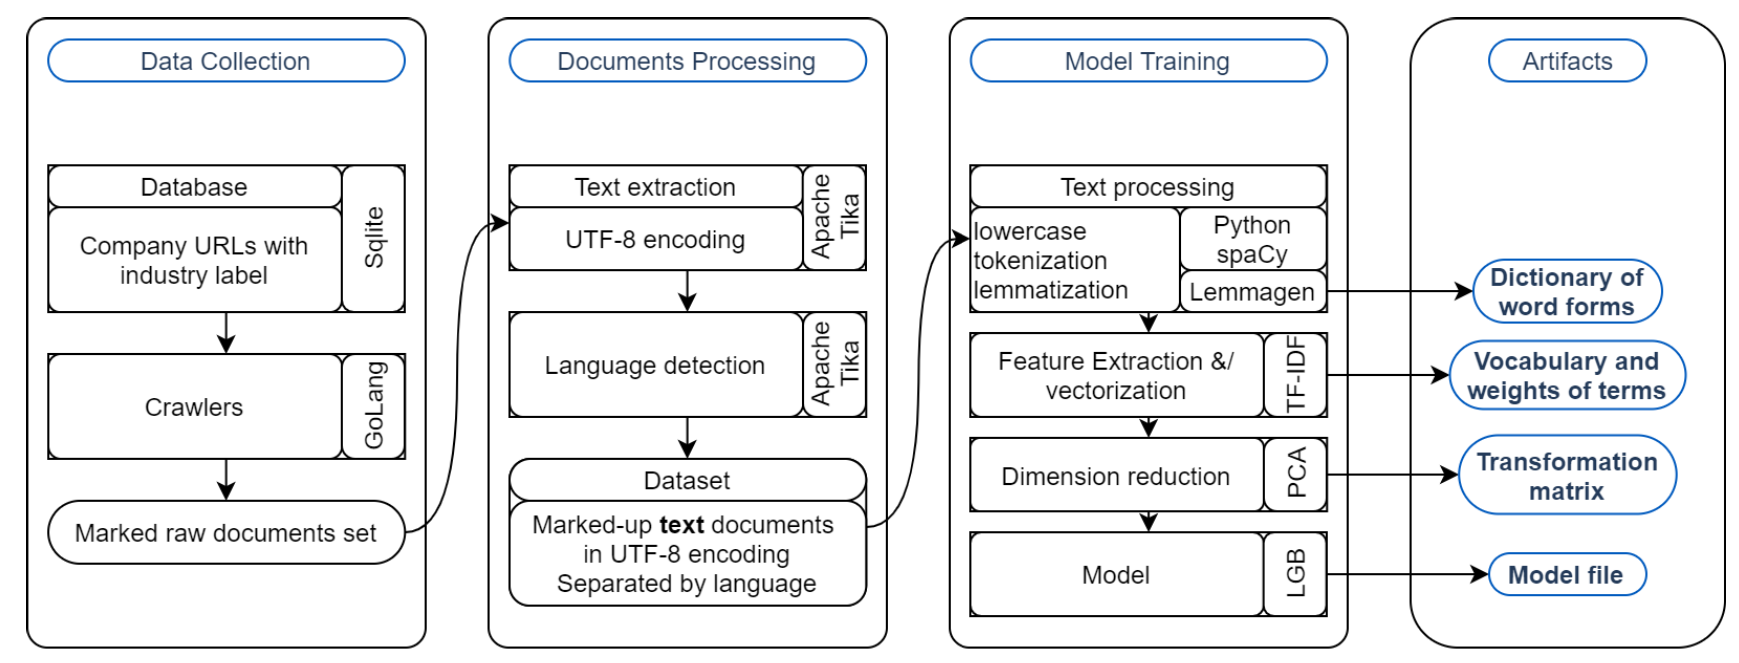
\includegraphics[width=\linewidth]{pipeline}
    \caption{Схематичное изображение процесса обучения}
    \label{fig:pipeline}
\end{figure}

Процесс обучения состоит из трех стадий:
\begin{enumerate}
    \item Сбор данных (data collection), см. \ref{sec:data-mining}.
    \item Обработка (processing) собранных документов, см. \ref{sec:preprocessing}.
    \item Обучение модели и сохранение артефактов, см. \ref{sec:training}.
\end{enumerate}
Каждая из этих стадий будет раскрыта подробнее в дальнейших секциях.

\section{Структура данных}
\subsection{Сырые данных}
В настоящей работе в качестве входных данных выступают документы, выгруженные из открытых источников в сети Интернет.
Данные представляют из себя веб-страницы, сохраненные локально в разнообразных форматах (HTML, PDF, .doc и другие).
Сопутствующий мультимедийный контент (видеозаписи, аудизаписи, картинки и т.п.) не сохраняется и не учитвается в модели.
Любой язык разметки, метаинформация, скрипты и таблицы стилей (в случае HTML) сохраняются в сырых документах <<как есть>>.

Все документы, участвующие в процессе, делятся на категории.
Категории заранее фиксированы и размечаются вручную.
Ниже приведен их список:
\label{categories}
\begin{itemize}
    \item Sales, Marketing and PR
    \item HR
    \item Finance and Banking
    \item IT, IT research and Development
    \item Manufacturing
    \item Medical and Paramedical
    \item Business and Corporate
    \item Legal
    \item Others
\end{itemize}

Разметка сырых данных фиксируется на уровне веб-сайта, т.е. \textbf{все} документы одного веб-сайта относятся к одинаковой категории.
Такой способ разметки является приближенным, поскольку один и тот же веб-сайт может содержать документы, относящиеся к различным тематикам (к примеру, медицинский сайт может содержать помимо мед.документов образцы договоров об оказании платных услуг).
\subsection{Данные для обучения}
Модель классификатора реализована на очищенных и нормализованных документах.
Данные для обучения представляют из себя набор файлов (по одному на каждую категорию из \ref{categories}), каждый из которых содержит множество документов.

Каждый документ в таком файле представляет из себя одну строку, которая заполнена словами в свой начальной форме, разделенными пробелом.
В таком формате данные предстают в человекочитаемом виде и то же время могут быть легко обрабтаны компьютером.

\section{Получение сырых данных}
\label{sec:data-mining}
\subsection{Общее описание \gls{crawler}}
\begin{wrapfigure}{r}{7cm}
    \centering
    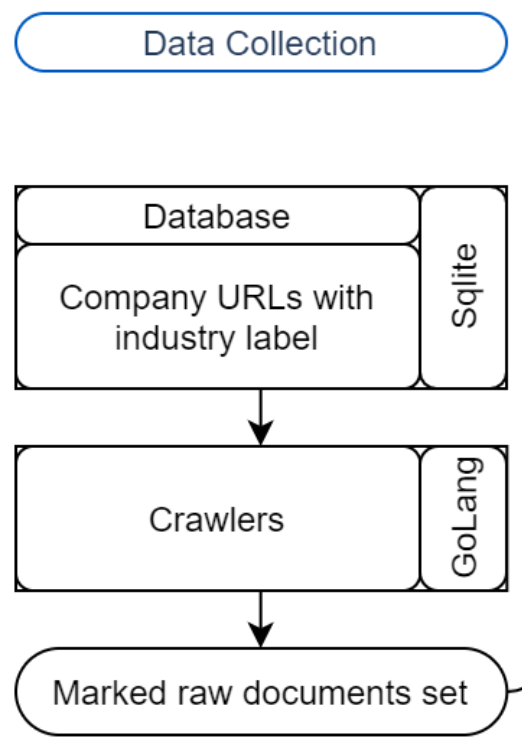
\includegraphics[width=\linewidth]{crawlers-pipeline}
    \caption{Архитектура \gls{crawler}}
    \label{fig:crawler-pipeline}
\end{wrapfigure}
Для получения документов была разработана программа для выгрузки веб-страниц (\gls{crawler}).
Для достижения большей производительности \gls{crawler} был написан на языке \gls{golang}, сочетающим высокую скорость работы и относительную простоту написания кода.

Схематично архитектура краулера показана на рис. \ref{fig:crawler-pipeline}.
На каждую поддерживаемую локализацию заводится своя база данных, содержащая ссылки сайтов, сгруппированные по категории.
Категории сайта записываются в базу данных вместе с множеством URL-адресов - пример этого изображен на рис. \ref{fig:crawler-db-head}.
Такая БД содержит немного данных, поэтому для простоты интеграции с \gls{golang} в качестве \acrshort{dbms} используется \gls{sqlite}.

\begin{figure}[h]
    \centering
    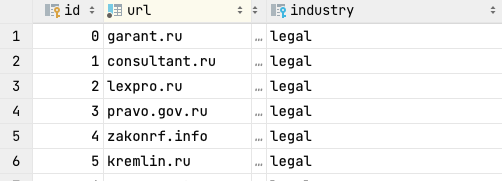
\includegraphics[width=0.8\linewidth]{crawler-db-head}
    \caption{Пример данных из БД краулера}
    \label{fig:crawler-db-head}
\end{figure}
Файл с заполненной базой данных поступает на вход программе \gls{crawler} (второй большой прямоугольник на \ref{fig:crawler-pipeline}), который запускет обход в глубину каждого URL-адреса.
В каждом выгруженном веб-сайте ищутся все возможные гиперссылки на другие страницы, и эти гиперссылки добавляются в очередь выгрузки.
Процесс продоложается до тех пор, пока вся очередь выгрузки для данного сайта не будет исчерпана, либо не будет достигнут лимит на количество загружаемых документов с одной страницы (\crawlerPageLimit).
\subsection{Типы используемых \gls{crawler}}
Существует несколько типов краулеров и подходов к их реализации \cite{cite:crawler-review}.
Помимо этого на стороне сайта возможно применение методов защиты от автоматической выгрузки \cite{cite:crawler-protection}.
Это, с одной стороны, создает некоторую вариативность, а с другой стороны -- обязывает иметь запасные варианты реализации сбора данных с веб-страниц.
С учетом данных факторов в настоящей работе используется три типа \gls{crawler}: \textit{google crawler}, \textit{colly crawler} \cite{cite:colly} и \textit{common index crawler} \cite{cite:common-crawl}.

Google \gls{crawler} напрямую запрашивает все документы с сайта через веб-поисковик \url{https://google.com}.
Этот метод весьма эффективен, т.к. полагается на собираемый Google индекс сайтов, но в то же время очень ограничен, т.к. \url{google.com} достаточно быстро начинает запрашивать CAPTCHA при запросе.
Обойти проверку CAPTCHA возможно несколькими способами, описанными, к примеру, в \cite{cite:captcha-bypass-1} и \cite{cite:captcha-bypass-2}.
Однако все эти способы требуют большие вычислительные мощности, что не удовлетворяло требованию о быстрой работе краулера.
Поэтому были разработы другие краулеры.

Common Index \gls{crawler} запрашивает копию страницы из интернет-архива \href{https://commoncrawl.org/}{Common Crawl}.
Это -- самый безотказный способ, т.к. веб-архив не требует ввода CAPTCHA и имеет нестрогие ограничения на количество запросов.
Тем не менее, архив может содержать не все страницы и скорость загрузки может быть ограничена из-за технических особенностей платформы.

Colly \gls{crawler} \cite{cite:colly} является самым продвинутым из описанных краулеров.
В то время как остальные \gls{crawler} полагаются на сторонние ресурсы, colly самостоятельно проходит по всем сайтам, выискивая все возможные гиперссылки на другие документы и проходя по ним в следующей итерации.
Такой алгоритм приводит к тому, что выгружаются практически все документы с сайта (кроме тех, что защищены авторизацией или проверками на ботов).
К сожалению, на больших сайтах алгоритм может достаточно долго блуждать по гиперссылкам.
Более того, нет никакой гарантии, что полученный граф обхода не содержит циклов, поэтому colly crawler может потенциально уйти в вечный цикл.
Для защиты от указанных проблем в данном \gls{crawler} выставлен лимит на время выполнения (\collyTimeLimit) и суммарный размер выгружаемых документов (\collySizeLimit).

Использование всех трех краулеров показало хорошие результаты -- по каждому языку было выгружено около \datasetSize сырых документов, что составило порядка \datasetDocs документов.

\section{Преобразование сырых данных в данные для модели}
\label{sec:preprocessing}
Как уже было сказано в \ref{chapter-1}, работа с текстом зачастую подразумевает его преобразование в вектора.
В данной работе указанный процесс, осуществляемый над сырыми данными, происходит в три стадии:
\begin{enumerate}
    \item Очистка текста от разметки и служебной информации.
    \item Выделение \textit{токенов} -- отдельных единиц языка в начальной форме.
    \item Непосредственное преобразование токенов каждого текста в вектора посредством \acrshort{tf-idf}.
\end{enumerate}
Остановимся кратко на каждом шаге.
\subsection{Очистка текста}
Для очистки текста от разметки и служебной информации используется программа \gls{apache} \gls{tika}.
Данная программа была выбрана по нескольким причинами:
\begin{enumerate}
    \item Скорость.
        \Gls{tika} быстро обрабатывает документы -- упомянутые 200 тысяч документов обрабатываются за 10 минут, что является хорошей скоростью по сравнению с остальными стадиями всего \gls{pipeline}.
    \item Зрелость продукта.
        \Gls{tika} разработывется фондом \Gls{apache}, что дает некоторые гарантии по стабильности продукта.
        Проект развивается с 2007 года и в настоящее время находится в зрелом состоянии.
    \item Поддержка большого числа форматов.
        На \href{https://tika.apache.org/1.10/formats.html}{официальной странице} используемой в проекте версии \gls{tika} заявляется поддержка более 20 форматов.
\end{enumerate}
С примерами данных после работы \Gls{tika} можно ознакомиться в листинге \ref{listing:tika-example}.
% TODO: (ruapyyj) рассказ про тику <- Thu Apr 21 13:26:19 2022
\subsection{Выделение токенов}
Для выделения токенов и приведения слов к нормальной форме (лемматизация, \gls{lemmatization}) существует несколько подходов \cite{cite:lemmatization-review}.
В данной работе рассматривалась работа на \gls{spacy} \cite{cite:spacy} и на \gls{nltk} \cite{cite:nltk}.

\gls{spacy} предоставляет богатый набор возможностей для обработки текста и построении на его основе комплексных \acrshort{ml} моделей.
В то же время данных фреймворк достаточно требователен к ресурсам, и даже частичное использование его языковых возможностей сопряжено с большими вычистительными затратами.
Несмотря на проведенные оптмизации и настройку \gls{pipeline} обработки текста, \gls{spacy} показал низкую скорость работы и стал лимитирующей стадией во всем \gls{pipeline} обучения.
Так, обработка одной локализации размером \datasetSize занимала у \gls{spacy} порядка трех дней, что сильно замедляло скорость разработки и проведения экспериментов.

Для расширения поддержки нескольких локализаций это стало недопустимым, и поэтому были проведены работы по поиску более производительных альтернатив, способных предоставить схожее качество лемматизации документов.
В качестве достойной альтернативы был выбран фреймворк \gls{nltk}, который смог полностью удовлетворить потребности по лемматизации.
Во-первых, \gls{nltk} имел встроенные алгоритмы \gls{lemmatization}, которые выдавали данные, схожие с выходными данными \gls{spacy}.
Во-вторых, скорость работы \gls{nltk} была на порядок выше скорости работы \gls{spacy}.
Уже упомянутый набор данных размером \datasetSize обрабатывался на \gls{nltk} за 20 минут, что было сопоставимо с остальными стадиями всего \gls{pipeline} обучения.

По итогу сравнения двух фреймворков был выбран \gls{nltk} в качестве токенизатора.
С примерам данных, получаемых в ходе его работы, можно ознакомиться в листинге \ref{listing:tokenizer-example}.
% TODO: (ruapyyj) рассказ про токенайзер <- Thu Apr 21 13:26:28 2022
% TODO: (ruapyyj) сравнение spacy и расскажи, как перевел все на nltk ради скорости <- Fri Apr 15 01:22:24 2022
\subsection{Преобразование в \acrshort{tf-idf}}
\label{par:tf-idf}
Для преобразования полученных после токенизации слов в векторы использется мера \acrfull{tf-idf} -- один из самых простых и первых способов векторного представления текста, который позволяет также изучать значимость слов \cite{cite:tf-idf-interpretation}.
Само преобразование просто: для каждого слова $t$ в документе $d$ из коллекции $D$ вычисляется мера:
\begin{equation}
    \label{eq:tf-idf}
    \text{tf-idf} (t, d, D) = \text{tf} (t, d) \cdot \text{idf} (t, D),
\end{equation}
которая состоит из двух компонент -- \acrfull{tf} и \acrfull{idf}.
\acrshort{tf} есть
\begin{equation}
    \label{eq:tf}
    \text{tf} (t, d) = \cfrac{n_t}{\sum_k n_k},
\end{equation}
где $n_t$ -- число вхождений слова $t$ в документ, а $\sum_k n_k$ представляет из себя общее число слов в данном документе.

\acrshort{idf} определяется как
\begin{equation}
    \label{eq:idf}
    \text{idf} (t, D) = \log \cfrac{|D|}{|\{d_i \in D | t \in d_i\}|},
\end{equation}
где $|D|$ -- общее число документов в коллекции, а знаменатель равен числу документов из коллекции $D$, в которых встречается $t$ (т.е. $n_t \neq 0$).

Данная метрика для слова из документа имеет интуитивную интерпретацию.
Ее \acrshort{tf} часть увеличивается тогда, когда слово чаще встречается в документе, но с другой стороны, слово должно встречаться часто именно в одном документе (согласно \eqref{eq:idf}) -- это не дает частым и не несущим смысла словами (таким как артикли) набирать большое значение \acrshort{tf-idf}.
Если слово встречается во всех документах, то его значимость в смысле \acrshort{tf-idf} уменьшается за счет уменьшения второго множителя в \eqref{eq:tf-idf}.

В настоящей работе используется реализация \acrshort{tf-idf} из библиотеки \gls{scikit-learn} \cite{cite:scikit-learn}.
\section{Модель \acrshort{ml} и ее обучение}
\label{sec:training}
Преобразованные и очищенные данные поступают классификатору, непосредственно решающему поставленную задачу \acrlong{mcc}.
В данной работе в качестве алгоритма классификации рассматривался градиентный бустинг над случайными деревьями, подробно описанная в \cite{cite:xgboost}.
Данная модель базируется на n принципах:
\begin{enumerate}
    \item Строится множество деревьев, из которого первое дерево строится по случайной подвыборке.
    \item На каждом этапе построения дерева решение о ветвлении принимается по случайному подмножеству признаков (метод случайных подпространств).
    \item Прогноз вероятности класса $k$ определяется как доля деревьев, проголосовавших за класс $k$.
    \item Каждое следующее дерево из леса обучается не на таргете $y$, а на ошибке предыдущего классификатора и градиенте этой ошибки (gradient boosting).
\end{enumerate}
Градиентый бустинг над случайными лесами -- очень популярный алгоритм в сфере \acrshort{ml}, его часто используют в качестве базового решения задачи.

Как уже было сказано в \ref{par:tf-idf}, в настоящей работе используется \acrshort{tf-idf}, который выдает вектор с количеством компонент, равным числу уникальных слов в наборе документов.
При используемых в работе данных это число может оказаться велико даже для случайных лесов, что может негативно сказаться затрачиваемом для обучения времени.
Поэтому перед обучением на векторе \acrshort{tf-idf} проводится уменьшение размерности методом \gls{pca}.
Кратко остановимся на сущности этого метода.

Интуитивно \gls{pca} может быть представлен как аппроксимация данных неким эллипсоидом.
Оси такого эллипсоида, обладающие наибольшей длиной, будут соответствовать наибольшей дисперсии.
Оставляя только первые $L < N$ осей, можно добиться снижения размерности.
$L$ будет подбираться так, чтобы доля объясненной дисперсии оставалась в допустимых рамках.
Задача \gls{pca} сводится к задаче о сингулярном разложении матрицы данных.
Задача о сингулярном разложении достаточно хорошо изучена, подробнее о ней можно почитать в \cite{cite:svd-1}, \cite{cite:svd-2}.
% TODO: (ruapyyj) мб побольше описать SVD и PCA? Вернись сюда, если текста не хватит <- Tue Apr 26 22:40:31 2022

В данной работе используется реализация \gls{pca} из библиотеки \gls{scikit-learn} с небольшой модификацией: вместо явного задания количества компонент $L$ выставляется порог на долю объясненной дисперсии, и количесто компонент выбирается так, чтобы выставленный порог был преодолен.
Такая реализация удобна при работе с несколькими локализациями, поскольку в общем случае для каждой отдельной локализации может потребоваться свое количество компонент.

Таким образом, модель обучается на векторизованных данных усеченной размерности в соответствии с замечаниями, упомянутыми выше.
По окончании описание леса, словарь \acrshort{tf-idf} и веса \gls{pca} выгружается, сохраняются в файл, версионируются (см. \ref{sec:dvc}) и отправляются в облачное хранилище (см. \ref{sec:gcloud}).
% TODO: (ruapyyj) здесь бы неплохо ссылку на то, сколько компонент в какой модели <- Tue Apr 26 22:40:02 2022

% Глава 3
%!TEX root = thesis.tex"`

\chapter{Автоматизация и версионирование экспериментов}
В развитии большинства \acrshort{ml}-проектов наступает момент перехода от стадии экспериментирования с прототипом модели к стадии построения системы, обладающей способностью к автоматическому запуску, наблюдаемостью и возможностью отслеживания ошибок. 
Данный процесс может быть весьма сложен, поскольку включает в себя применение некоторых практик \gls{swe} и \gls{devops}.
Его изложению и будут посвящены дальнейшие секции.
\section{Технический долг в \acrshort{ml} системах}
\label{sec:ml-debt}
В статье \cite{cite:ml-debt} подробно описан так называемый технической долг в применении к \acrshort{ml}-проектам.
Многие из указанных авторами проблем были характерны и для настоящей работы:
\begin{enumerate}
    \item Зависимость от нестабильных данных.
        Данные, используемые во всем процессе или отдельных экспериментах, могут храниться в ненадежном месте или не быть доступными воспроизводимым способом.
    \item Отсутствие статических проверок на наличие данных.
        Подразумевается проверка на наличие всех необходимых данных перед запуском каждой стадии процесса.
    \item <<Спагетти-код>> -- основной код перемешан с большим количеством связывающего кода, не несущего существенного смысла, но необходимого для соединения компонент воедино.
    \item Тупиковые экспериментальные ветвления, при которых в коде присутствует множество ответвлений для некоторых экспериментов, которые были заброшены и в актуальной версии кода приводят соответствующее ответвление в нерабочее состояние.
    \item Отсутствие отслеживания конфигурации всего \gls{pipeline}.
    Настройки модели должны быть явно выделены, должны версионироваться и быть простыми для визуального понимания человеком.
    \item Мониторинг и логгирование.
        Модель и \gls{pipeline} должны иметь систему журналирования действий, систему отслеживания ошибок и отклонений от ожидаемого поведения.
    \item Воспроизводимость.
        Каждый разработчик должен быть в состоянии воспроизвести то же состояние \gls{pipeline}, что и другой разработчик, с теми же выходными данными и состоянием кода.
    \item Слабая способность к управлению множественными процессами.
        При запуске большого количества моделей должна быть возможность следить за каждой из них с учетом описанных выше требований.
\end{enumerate}

Данные проблемы частично дублируют проблемы, возникающие в классическом \gls{swe}.
Так, <<спагтти-код>> встречается не только в среде \acrshort{ml}, но и в классической разработке ПО.
Отслеживание конфигурации важно в любом проекте, в той или иной степени утилизирующем хранение настроек в отдельных файлах.
Мониторинг и логгирование являются основными компонентами любого зрелого программного комплекса, и для них к моменту написания настоящей работы уже имеется накопленная экспертиза.
Тем не менее, в случае задач машинного обучения требуется модификация существующих подходов, поскольку работа всей системы зависит не только от логики программного кода, но и от качества входных данных.

Каждая из этих проблем была решена в рамках настоящей работы.
Изложению способа решения и достигнутых результатов будут посвящены дальнейшие секции.
\section{Автоматизация \gls{pipeline} обучения}
\label{sec:dvc-pipeline}
Выстраивание системы автоматического запуска всех шагов процесса обучения -- одна из первых задач на пути решения описанных в \ref{sec:ml-debt} проблем.
Для построения автоматизации такого рода был выбран фреймворк \gls{dvc} \cite{cite:dvc}.
На момент написания данной работы была актуальна версия 2.10.2, и дальнейшее изложение будет строиться на основе нее.

\Gls{dvc} оперирует в абстракциях <<стадий>> (\textit{stage}) -- некоторых действиях над данными.
Каждая такая стадия имеет входные данные (\textit{deps}), выходные данные (\textit{outs}), параметры, от которых стадия зависит (\textit{params}), и опционально может содержать метрики (\textit{metrics}) и графики (\textit{plots}).
Основная идея состоит в том, чтобы каждая стадия была зависима либо от выхода предыдущей стадии, либо от <<сырых>> данных, явно прописанных как часть \gls{pipeline}.
При таком подходе становится возможным представить весь процесс работы \acrshort{ml}-проекта как проход по \textit{направленному ацикличному графу}, называемому также \acrfull{dag}.
Визуальная иллюстрация приведена на рисунке \ref{fig:dvc-pipeline}.

\begin{figure}[!h]
    \centering
    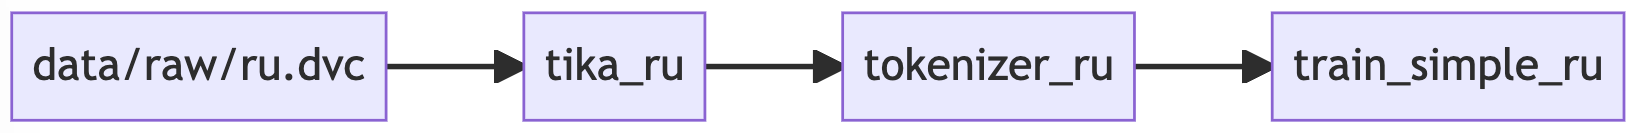
\includegraphics[width=\linewidth]{dvc-pipeline}
    \caption{Визуальное представление \acrshort{dag} обучения}
    \label{fig:dvc-pipeline}
\end{figure}

Приведенный на рисунке \ref{fig:dvc-pipeline} граф был построен по следующим правилам:
\begin{enumerate}
    \item Каждая стадия и каждый явно прописанный входной файл представляются вершинами графа.
    \item Для каждой стадии анализируется список ее зависимостей (\textit{deps}).
        Если эти зависимости удовлетворяются одной из описанных стадий (проверются выходные файлы стадии) или входным файлом, указанном наравне со стадиями, то проводится ребро между двумя стадиями, направленное в стороне зависимой.
        Если зависимости не удовлетворяются, то выдается ошибка запуска.
    \item Проверяется наличие циклов в полученном графе.
        Если они обнаружены, то выдается ошибка запуска.
\end{enumerate}
Построенный таким образом граф не только задает последовательность операций, но и явно описывает все входные и выходные данные.
Это позволяет настроить \textit{статистические проверки на наличие данных}, которые описаны среди проблем в \ref{sec:ml-debt}.
Помимо этого, описание всего процесса в едином графе вычислений дает возможность управлять процессом и производить его масштабирование, добавляя тем самым \textit{способность к управлению множественными процессами}.

Помимо выстраивания \gls{pipeline}, \gls{dvc} предоставляет широкий спектр других возможности для автоматизации задач машинного обучения.
К примеру, возможно создавать так называемые <<эксперименты>>, которые представляют из себя воспроизводимый запуск всего \gls{pipeline} с измениями в конфигурации и/или исходном коде моделей.
Помимо этого поддерживается экспериментальная поддержка работы на удаленной машине (см. документацию \cite{cite:dvc}).
При таком подходе компьютер разработчика выступает в роли т.н. тонкого клиента -- весь код редактируется локально, а фактические вычисления осуществляются на удаленном компьютере.

Разделение кода на стадии, предлагаемое в \gls{dvc}, позволяет выстроить четкое разделение процесса на состоявляющие компоненты, избавляя от описанной в \ref{sec:ml-debt} проблемы <<спагетти>>-кода: вместо единого большого файла с набором инструкций будет порождено несколько небольших скриптов, выполняющих одну задачу, и выполняющих ее хорошо.
В настоящей работе удалось успешно осуществить такое разделение.
Первоначальная версия модели, выполненная в едином файле \gls{jupyter-notebook}, была разбита на множество отдельных скриптов, каждый из которых расширял и обобщал существующую функциональность исходного прототипа.
\section{Версионирование данных, артефактов и визуализация метрик}
\label{sec:dvc}
% TODO: (ruapyyj) ну, тоже dvc <- Tue Apr 26 23:11:29 2022

\subsection{Проблемы при версионировании данных}
\label{sec:dvc-versioning-problems}
С теоретической точки зрения версионирование данных ничем не отличается от версионирования исходного кода.
Ожидается, что система хранения данных способна возвращаться к любой заранее отмеченной версии, хранить эти версии в удаленном хранилище и иметь возможность переключаться между различными версиями.
Практическая реализация, тем не менее, осложняется по нескольким причинам.

Во-первых, существующие системы контроля версий (\acrlong{vcs}) изначально создавались для хранения файлов исходного кода, имеющих малый размер, что в большинстве случаев определило их архитектуру.
Так, используемый в данной работе \gls{git} по умолчанию выгружает полную копию всех версий всех файлов, находящихся под отслеживанием, что не является проблемой для <<легких>> файлов (например, небольших документов, исходного кода), но совершенно неприменимо для больших файлов с данными, используемых в \acrshort{ml}-проектах.

Вторая причина состоит в том, что большинство \acrshort{vcs} реализуют собственные системы для физического хранения версий объектов -- к примеру, \gls{git} сохраняет файлы в директории \texttt{.git/}, полученной от сервера с исходными кодами.
Собственные реализации хранилища могут быть применимы и для данных большего размера, но зачастую под хранение объектов значительного объема используются специализированные под такую задачу решения (например, \gls{s3}-хранилища, система \gls{hadoop} с ее распределенной файловой системой \gls{hdfs} и т.п.).

Описанные проблемы решены в \gls{dvc}.
Вместо версионирования самих файлов с данными \gls{dvc} отправляет в \acrshort{vcs} файл с хеш-суммой файла (по умолчанию используется MD5).
Сам файл отправляется в кэш (может храниться как локально, так и на \gls{hdfs}).
Каждая версия файла таким образом будет представлять из себя пару (\textit{файл с хешом}, \textit{файл с содержимым}), где последний исключается из отслеживания \gls{vcs}.
Когда необходимо переключиться между версиями, соответствующий хеш-сумме файл достается из кэша и перекладывается в рабочую область.

Кэш с файлами допускает хранение на удаленных серверах.
В \gls{dvc} реализована поддержка большого количества хранилищ: \acrshort{sshfs}, \gls{hdfs}, \gls{s3}, \gls{webdav} и других (полный список доступен в \href{https://dvc.org/doc/command-reference/remote/add#supported-storage-types}{документации}).
Такой подход позволяет использовать уже существующую инфраструктуру для задач версионирования.

\subsection{Решение в рамках данной работы}
В \ref{sec:dvc-pipeline} было указано, что каждая стадия имеет явно заданные входные и выходные данные.
Помимо \textit{наблюдаемости} данных (возможности в любой момент знать, какие данные для чего используются) это позволяет вести их учет, версионировать и сохранять в надежных хранилищах (например, в \gls{s3}).
Описанная возможность успешно реализована в настоящей работе силами фреймворка \gls{dvc}.

Вход и выход каждой стадии версионируется упомянутым фреймворком в соответствии с процедурой, описанной в \ref{sec:dvc-versioning-problems}.
Кэш объектов хранится локально на диске большого объема и на удаленном \gls{s3}-хранилище (в целях обеспечения отказоустойчивости).

Подобная организация позволяет решить несколько проблем из \ref{sec:ml-debt}.
Во-первых, все зависимости от данных становятся \textit{стабильными} за счет того, чтобы данные версионируются, имеют привязку к версии кода (\gls{dvc} достигает это через добавление файла с хешом в \gls{vcs}) и надежно хранятся в удаленном хранилище.

Во-вторых, появляется \textit{воспроизводимость} процесса -- каждый разработчик в состоянии запустить весь \gls{pipeline} с теми же входными данными и версиями кода, что и были в прошлых запусках.
Здесь стоит заметить, что для \textit{полной воспроизводимости} необходимо также убедиться, что каждый скрипт при одинаковых входных данных будет производить одинаковые выходы от запуска к запуску.
В настоящей работе это было достигнуто фиксированием random seed и значения текущего времени во всех зависимых от времени в инструкциях (подробнее о техниках воспроизводимости описано в \cite{cite:ml-reproducibility}).

В-третьих, указание файла настроек в качестве зависимости привело к \textit{отслеживанию конфигурации} всего \gls{pipeline} и автоматическому перерасчету релеватных стадий при изменениях в настройках.
Для получения всех преимуществ подобного отслеживания в настоящей работе все настройки всего \gls{pipeline} обучения (кроме сбора данных краулерами) были вынесены в единый файл (концепция <<single source of truth>>).
Этот файл версионируется, используя \gls{git}, и изменения в нем служат индикатором для перезапуска тех стадий, которые зависят от измененных параметров.

Стадия обучения модели настроена на выгрузку весов и внутренней структуры леса в отдельные файлы, каждый из которых прописан в настройках \gls{dvc} -- благодаря этому артефакты обучения подлежат версионированию и хранению наравне с данными.

\subsection{Визуализация в \gls{dvc}}
Особое внимание стоит обратить на работу с метриками и графиками.
\Gls{dvc} позволяет не только версионировать метрики и данные для графиков, но и сравнивать их между различными ревизиями.

Для сравнения метрик между собой их необходимо выгрузить в файл в одном из поддерживаемых форматов (в работе используется \texttt{JSON}) и описать файл в \gls{dvc} \gls{pipeline}.
После этого появится возможность сравнивать различные версии этого файла между собой и строить отчеты в формате Markdown.
Такое сравнение удобно, когда требуется быстро понять результат тех или иных изменений в коде или данных.
Формат метрик никак не ограничивается -- возможно хранить любые JSON-сериализуемые пары <<ключ-значение>>.
Пример отчета по метрикам со сравнением между ревизиями показан в таблице \ref{table:dvc-metrics-diff}.

\begin{table}[!ht]
    \centering
    \begin{tabular}{|l|l|l|l|l|}
    \hline
        Path & Metric & main & 0b257f19 & Change \\ \hline
        it/metrics.json & Businises\&Corporate.f1-score & 0.96526 & 0.96487 & -0.00039 \\ \hline
        it/metrics.json & Businises\&Corporate.precision & 0.96487 & 0.96412 & -0.00075 \\ \hline
        it/metrics.json & Businises\&Corporate.recall & 0.96566 & 0.96562 & -3e-05 \\ \hline
        it/metrics.json & Businises\&Corporate.support & 1223 & 1280 & 57 \\ \hline
        it/metrics.json & Finance\&Banking.f1-score & 0.99403 & 0.99379 & -0.00023 \\ \hline
        it/metrics.json & Finance\&Banking.precision & 0.99289 & 0.99346 & 0.00057 \\ \hline
        it/metrics.json & Finance\&Banking.recall & 0.99517 & 0.99413 & -0.00104 \\ \hline
        it/metrics.json & Finance\&Banking.support & 4347 & 4430 & 83 \\ \hline
    \end{tabular}
    \caption{Пример сравнения метрик между ревизиями}
    \label{table:dvc-metrics-diff}
\end{table}

\begin{figure}[!h]
    \centering
    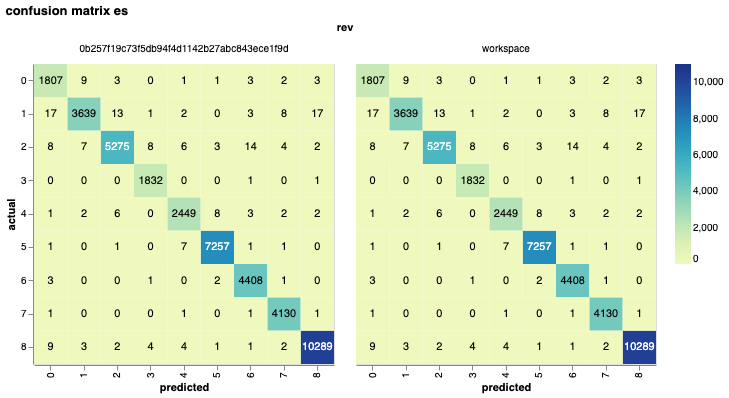
\includegraphics[width=\linewidth]{dvc-plots-diff}
    \caption{Пример сравнения confusion matrix между ревизиями. В заголовке каждого графика указывается ревизия, по которой тот был отрисован. Метки классов представлены числами.}
    \label{fig:dvc-plots-diff}
\end{figure}
\begin{figure}[!ht]
    \centering
    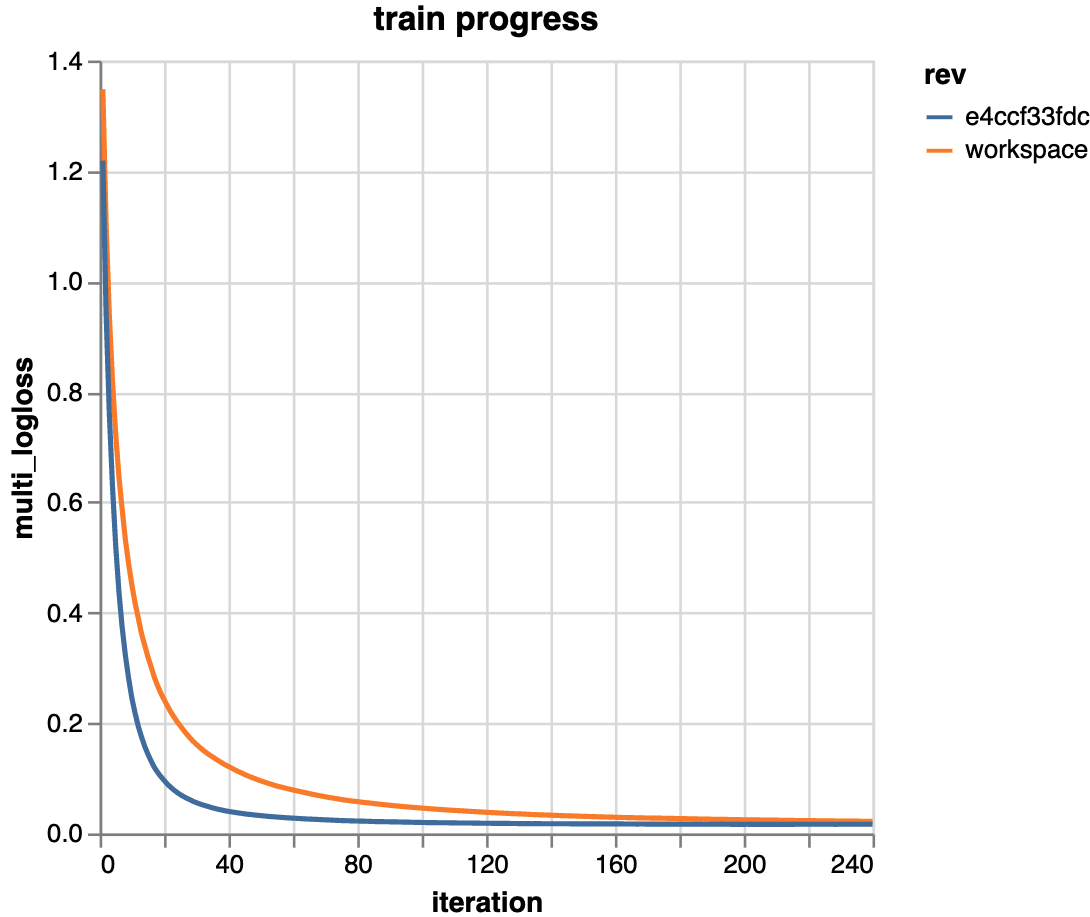
\includegraphics[width=0.9\linewidth]{dvc-plots-diff-real}
    \caption{Пример отображения различий в графиках между ревизиями}
    \label{fig:dvc-plots-diff-real}
\end{figure}
В случае графиков имеется аналогичная возможность сравнения ревизий.
Требуется выгрузить данные для построения графиков в отдельный файл, описать его в \gls{dvc} \gls{pipeline}, после чего появится возможность отрисовки графиков двух версий на одном полотне.
Пример этого представлен на рис. \ref{fig:dvc-plots-diff}.

При отрисовке кривых обе отображаются на одном графике для простоты визуального сравнения -- как это показано на рисунке \ref{fig:dvc-plots-diff-real}.

На рисунке \ref{fig:dvc-plots-labels} можно видеть confusion matrix с текстовым указанием классов.
\begin{figure}[!ht]
    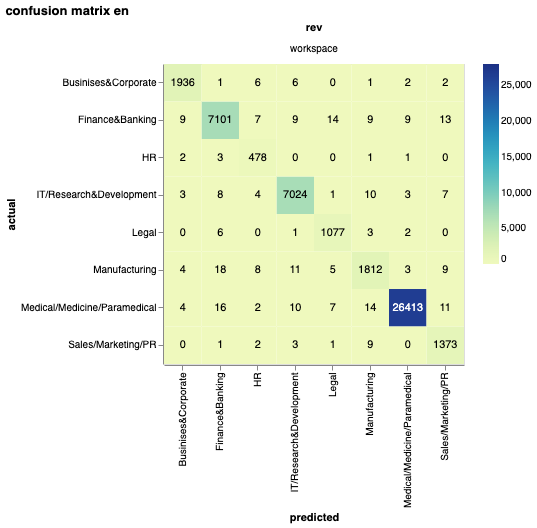
\includegraphics[width=\linewidth]{dvc-plots-labels}
    \caption{Пример confusion matrix с текстовым указанием классов}
    \label{fig:dvc-plots-labels}
\end{figure}

Существует веб-сайт, в котором возможно получать все упомянутые визуализации в режиме онлайн.
Это DVC Studio, продукт от создателей \gls{dvc}.
Проект, описываемый в настоящей работе, можно найти \href{https://studio.iterative.ai/user/alekseik1/views/dataclassification-crawler-e1vtfsj7dv}{здесь}, а на рисунке \ref{fig:studio} изображен пример работы с сайтом.

\begin{figure}[!h]
    \centering
    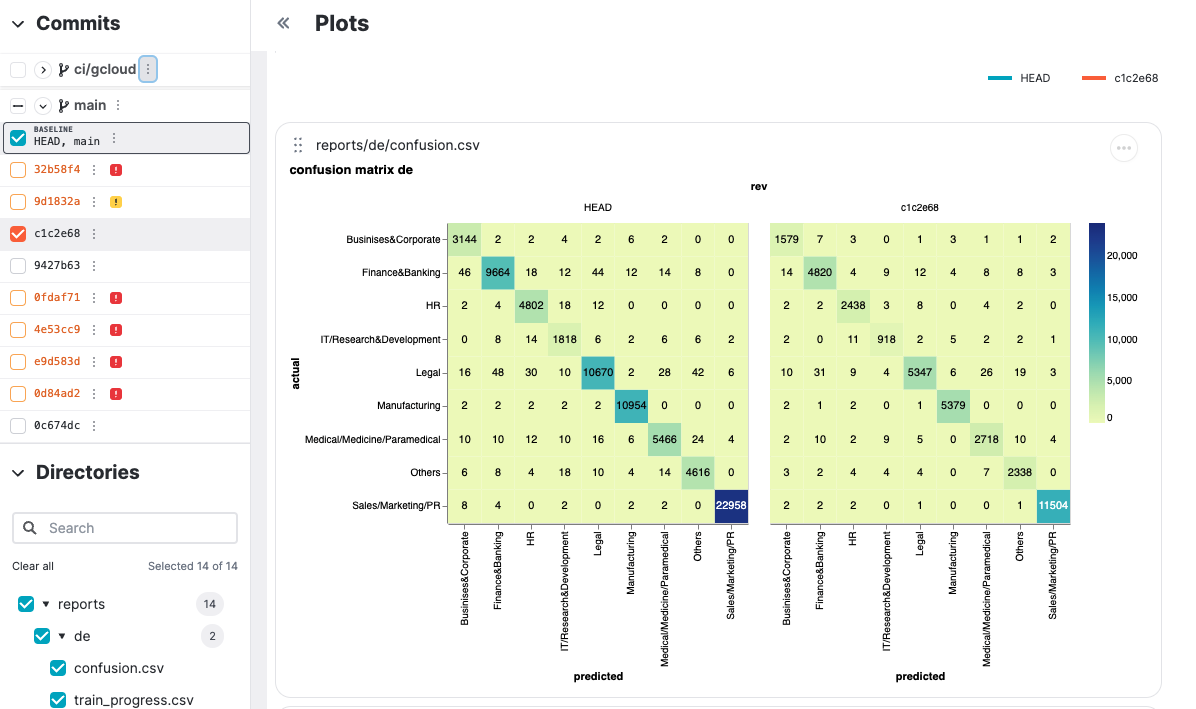
\includegraphics[width=\linewidth]{studio}
    \caption{Интерфейс веб-страницы с визуализацией метрик}
    \label{fig:studio}
\end{figure}
\section{Журналирование, хранение старых экспериментов}
Из описанных в \ref{sec:ml-debt} проблем остаются \textit{тупиковых экспериментальных ветвлений} и \textit{мониторинга с журналированием}.
Первая из них решена в данной работе использованием тегов в \gls{git} -- на каждый эксперимент выставляется тег, но изменения кода модели не вливаются в основную ветку при отсутствии успеха.
В таком случае основная ветка остается свободной от остатков неудачных экспериментов и тупиковых условных переходов внутри кода.
К неудавшемуся эксперименту всегда будет возможно вернуться, поскольку использованные в нем данные и код версионируются \gls{dvc}.

Вторая проблема решена частично -- в код модели встроено обильное логгирование.
Логи складируются в файлы, разделенные отдельными запусками, и каждая запись имеет унифицированный формат, что облегчит последующую обработку автоматическими инструментами по работе с журналами.
Примеры таких инструментов приведены в секции \ref{sec:future}.

Хранение старых экспериментов реализовано силами \gls{dvc}.
Встроенная в этот инструмент возможность хранить артефакты каждой стадии \gls{pipeline} с привязкой к коммиту \gls{git} активно используется в настоящей работе.
А использование \gls{s3}-хранилища дает возможность надежно хранить артефакты любой версии.

Таким образом, использование в данной работе \gls{dvc} и продвинутых возможностей \gls{git} позволило решить все проблемы, намеченные в \ref{sec:ml-debt}.
Подкрепленная такими возможностями, построенная на одной локализации модель допустила обобщение, в результате чего удалось автоматизировать процесс обучения на новых данных, обобщить его на другие языки и упростить процесс коллаборации с другими участниками проекта.
\section{Дальнейшие планы по работе}
\label{sec:future}
Проведенные в настоящей работе усилия по автоматизации значительно приблизили первоначальный прототип системы классификации документов к состоянию самообучающейся модели.
Тем не менее, возможны дальнейшие улучшения, намеченные к реализации в будущей работе.
Ниже кратко рассмотрены планы по дальнейшей работе.
    \subsection{Выстроение обучения в \gls{cicd}}
    Предполагается выполнять тестовый запуск всего пайплайна обучения на сервере при каждом успешном Merge Request в основную ветку, как показано на \ref{fig:cicd}.
    \begin{figure}[h]
        \centering
        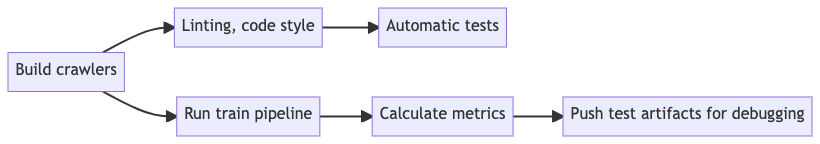
\includegraphics[width=\linewidth]{cicd}
        \caption{Предполагаемая настройка \gls{cicd} пайплайна}
        \label{fig:cicd}
    \end{figure}
    На остальных ветках \gls{pipeline} обучения будет выполняться над небольшим набором данных, чтобы быстрее получить и передать разработчикам обратную связь.
    Это позволит ускорить итерации разработки и автоматизировать переобучение при обновлении кодовой базы.

    На момент написания работы данная задача частично решена.
    При каждом коммите происходит запуск \gls{pipeline} обучения на небольшом наборе данных с целью определить работоспособность кода.
    Тем не менее, полноценное тестирование на всем датасете, равно как и сравнение метрик между ревизиями, все еще требуют разработки и имплементации.

    Для реализации такой задачи хорошо подойдет инструмент \href{https://cml.dev/}{CML}
    \subsection{Валидация входных данных при обучении}
    При обучении модели имеет смысл исключать выбросы, поскольку ее качество может значительно пострадать при наличии существенных отклонений в данных.
    Разработка алгоритма определения неподходящих для обучения данных и последующая автоматизация этого алгоритма позволит увеличить метрики качества модели без существенного изменения ее сути.
    \subsection{Автоматическое детектирование серьезных отклонений в предсказаниях}
    Текущая реализация модели может предсказывать вероятность каждого из классов.
    Имеет смысл сохранять те документы, на которых модель имеет близкие вероятности у двух различных классов -- документы, в которых модель <<не уверена>> в предсказаниях.
    Впоследствии такие примеры следует проанализировать, дабы извлечь закономерность появления неоднозначности ответа модели.

    Предположительно данная задача может быть решена с использованием инструмента от \href{https://evidentlyai.com/}{evidently AI}.
    \subsection{Улучшение ручной разметки входных данных}
    На этапе прототипирования был выбран очень простой алгоритм разметки: если сайт имеет тематику $X$, то всего документы помечаются как имеющие тематику $X$.
    Такая разметка проста в реализации, но не является до конца корректной -- поэтому ее улучшение может повысить качество модели.

    Среди возможных способов стоит отметить применение кластеризации документов, размечивание с привлечением экспертов и использование более сложных моделей (или ансамблей) для исключения ошибок текущей разметки.
    \subsection{Централизованная система логгирования}
    Хранение и анализ логов полезно для работы над ошибками в программе и поиска узких мест всего процесса.
    По мере роста проекта количество журналов значительно растет, и возникает нужда в автоматических средствах хранения, поиска и обработки логов.
    На момент написания работы логи каждого шага всего процесса обучения пишутся в файлы, хранимые локально на сервере запуска (описанном в приложении \ref{sec:gcloud}).

    Для решения такой проблемы можно использовать одно из готовых решений -- к примеру, стек \gls{elk} или его простой аналог \href{https://www.graylog.org/}{Graylog}.


% Заключение
%!TEX root = thesis.tex"`

\conclusion

В даной работе получены следующие результаты:

\begin{enumerate}
    \item Прототип модели классификации документов для одной локализации выведен в продуктив, на его основе разработан \gls{pipeline} обучения от начала до конца.
    \item Модель обобщена на другие локализации (см. таблицу \ref{table:supported_locales}) с единый пайплайном.
    \item Выстроен процесс разработки, настроена система ведения журналов и поиска неисправностей кода.
    \item Автоматизирован процесс дообучения модели на новых данных.
    % \item Получены аналитические выражения для вторых производных термодинамического потенциала и термодинамических коэффициентов \acrshort{ifg}.
    % \item Получены асимптотические выражения для всех термодинамических функций \acrshort{ifg} в пределе низких и высоких температур.
    % \item Разработана общедоступная программная реализация для модели \acrshort{ifg} на языке \Gls{python}.
    % \item Получен гамильтониан изотропной модели \acrshort{veg}.
    % \item Разработан алгоритм программной реализации \acrshort{mfp} для модели \acrshort{veg}.
\end{enumerate}

В дальнейшем планируется расширять список поддерживаемых локализаций, добавлять систему контроля качества и автоматизировать ее посредством \gls{cicd}.

\begin{table}[h]
    \centering
    \begin{tabular}{|c|c|c|}
        \hline
                 & precision & recall  \\ \hline
        German   & 0.98520   & 0.97661 \\ \hline
        English  & 0.95502   & 0.95358 \\ \hline
        Spanish  & 0.99263   & 0.99159 \\ \hline
        French   & 0.97535   & 0.97113 \\ \hline
        Italian  & 0.97212   & 0.95854 \\ \hline
        Japanese & 0.95297   & 0.91297 \\ \hline
        Russian  & 0.99175   & 0.99071 \\ \hline
    \end{tabular}
    \caption{Таблица поддерживаемых локализаций}
    \label{table:supported_locales}
\end{table}


% Список литературы
\printbibliography[heading=bibintoc]

% Приложения
\appendix
%!TEX root = thesis.tex"`
\chapter{Описание инфраструктуры}
\label{sec:gcloud}
В настоящей работе инфраструктура развертывания проекта была выполнена на базе серверов облачного провайдера \href{https://cloud.google.com}{Google Cloud}.

Система обучения развернута на \gls{vps} машине, для долгосрочного хранения данных и артефактов используется \gls{s3}-хранилище.

Характеристики \gls{vps} машины представлены ниже:

\begin{table}[!h]
    \centering
    \begin{tabular}{|l|c|}
        \hline
        Тип               & e2-standard-8      \\ \hline
        CPU Platform      & Intel Broadwell    \\ \hline
        Ядер              & 8                  \\ \hline
        RAM               & 32 \acrshort{gb}   \\ \hline
        Диск для загрузки & 100 \acrshort{gb}  \\ \hline
        Диск для хранения & 1536 \acrshort{gb} \\ \hline
        Файловая система  & XFS                \\ \hline
        ОС                & Debian 11          \\ \hline
    \end{tabular}
    \caption{Характеристики основной машины}
    \label{tab:vps-info}
\end{table}
% \chapter{Пример расчета\\ термодинамических свойств \texorpdfstring{\acrshort{ifg}}{ИФГ}}
% Модуль легко ставится через \Gls{pypi}:
% \begin{minted}{bash}
% $ pip install numpy
% $ pip install ifg
% \end{minted}

% Основной функционал содержится в классе \texttt{IfgCalculator}.
% \begin{minted}{Python}
% from ifg import IfgCalculator
% import numpy as np
% specific_volumes = [0.33, 1., 10.,]
% temperatures = np.linspace(1e-4, 1e4, 10**6)
% calculator = IfgCalculator(
%     temperatures=temperatures,
%     specific_volumes=specific_volumes,
%     input_in_si=False,  # False даст в атомной системе
%     output_in_si=False
% )
% \end{minted}
% После этого все свойства будут доступны как поля экземпляра \texttt{calculator}:
% \begin{minted}{Python}
% >>> calculator.p
% array([[1.21465823e+01, 1.91415600e+00, 4.12392425e-02],
%        [1.21466330e+01, 1.91419106e+00, 4.12555143e-02],
%        [1.21467832e+01, 1.91429487e+00, 4.13036646e-02],
%        ...,
%        [3.03030975e+04, 9.99999392e+03, 9.99998139e+02],
%        [3.03031278e+04, 1.00000039e+04, 9.99999139e+02],
%        [3.03031581e+04, 1.00000139e+04, 1.00000014e+03]])
% >>> calculator.C_P
% array([[4.92449475e-05, 1.03122265e-04, 4.78651124e-04],
%        [4.97374654e-03, 1.04153735e-02, 4.83453163e-02],
%        [9.89825789e-03, 2.07277142e-02, 9.62203561e-02],
%        ...,
%        [2.49998418e+00, 2.49999478e+00, 2.49999948e+00],
%        [2.49998418e+00, 2.49999478e+00, 2.49999948e+00],
%        [2.49998418e+00, 2.49999478e+00, 2.49999948e+00]])
% \end{minted}
% Во втором примере видим, как теплоемкость $C_P$ стремится к $5/2$ при высоких температурах ---~ ожидаемое поведение для \acrshort{ifg}.

% Можно также проверить, что давление стремится к конечному пределу при низких температурах.
% Изменим входные данные:
% \begin{minted}{Python}
% temperatures = np.linspace(1e-10, 1e-8, 10**4)
% calculator = IfgCalculator(
%     temperatures=temperatures,
%     specific_volumes=specific_volumes,
%     input_in_si=False,
%     output_in_si=False
% )
% \end{minted}
% А затем запустим расчет давления:
% \begin{minted}{Python}
% >>> calculator.p
% array([[12.14658227,  1.914156  ,  0.04123924],
%        [12.14658227,  1.914156  ,  0.04123924],
%        [12.14658227,  1.914156  ,  0.04123924],
%        ...,
%        [12.14658227,  1.914156  ,  0.04123924],
%        [12.14658227,  1.914156  ,  0.04123924],
%        [12.14658227,  1.914156  ,  0.04123924]])
% \end{minted}
% Получены конечные пределы.

% Больше примеров можно найти по ссылке \url{https://ifg-py.readthedocs.io/en/latest/class_desc.html}.
% Код графиков \ref{fig:chemical_potential}, \ref{fig:heat_capacity}, \ref{fig:sound_velocity} доступен в репозитории: \url{https://github.com/alekseik1/ifg-py/tree/master/examples/plots}.
\appendix
\chapter{Примеры данных после каждой стадии}
\begin{listing}[!ht]
\begin{minted}{json}
{
  "metadata": {
    "Content-Encoding": "UTF-8",
    "Content-Language": "en-GB",
    "Content-Type": "text/html; charset=UTF-8",
    "X-Parsed-By": [
      "org.apache.tika.parser.DefaultParser",
      "org.apache.tika.parser.html.HtmlParser"
    ],
    "dc:title": "Amex - Giving Airmiles a Human Touch",
    "og:site_name": "BBH Global",
    "og:title": "Amex - Giving Airmiles a Human Touch",
    "og:type": "website",
    "og:url": "https://www.bartleboglehegarty.com/...",
    "title": "Amex - Giving Airmiles a Human Touch",
    "language": "en"
  },
  "content": "\n\nAmex - Giving Airmiles a Human Touch\n...",
  "status": 200
}
\end{minted}
\caption{Пример данных после \gls{tika}}
\label{listing:tika-example}
\end{listing}

\begin{listing}[!ht]
\begin{minted}{text}
home the richards group about u culture our people practice ...
omnicom group global marketing communication omnicom group ...
legal the richards group about u culture our people practice ...
interpublic group ipg ipg our value diversity and inclusion ... 
\end{minted}
\caption{Пример данных после \gls{nltk}}
\label{listing:tokenizer-example}
\end{listing}


\end{document}
